% This file was created by tikzplotlib v0.9.8.
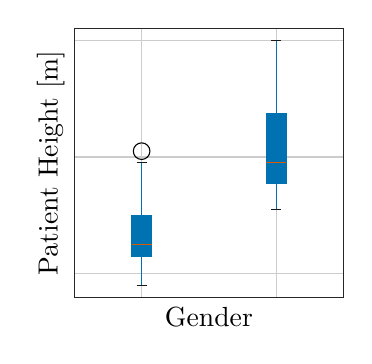
\begin{tikzpicture}

\definecolor{color0}{rgb}{0,0.447058823529412,0.698039215686274}
\definecolor{color1}{rgb}{0.835294117647059,0.368627450980392,0}

\begin{axis}[
axis line style={white!15!black},
height=5cm,
tick align=outside,
width=5cm,
x grid style={white!80!black},
xlabel={Gender},
xmajorgrids,
xmajorticks=false,
xmin=0.5, xmax=2.5,
xtick style={color=white!15!black},
xtick={1,2},
xticklabels={F(39),M(15)},
y grid style={white!80!black},
ylabel={Patient Height [m]},
ymajorgrids,
ymajorticks=false,
ymin=1.559, ymax=2.021,
ytick style={color=white!15!black}
]
\addplot [color0, opacity=1]
table {%
1 1.63
1 1.58
};
\addplot [color0, opacity=1]
table {%
1 1.7
1 1.79
};
\addplot [white!10!black, opacity=1]
table {%
0.9625 1.58
1.0375 1.58
};
\addplot [white!10!black, opacity=1]
table {%
0.9625 1.79
1.0375 1.79
};
\addplot [black, mark=o, mark size=3, mark options={solid,fill opacity=0}, only marks]
table {%
1 1.81
};
\addplot [color0, opacity=1]
table {%
2 1.755
2 1.71
};
\addplot [color0, opacity=1]
table {%
2 1.875
2 2
};
\addplot [white!10!black, opacity=1]
table {%
1.9625 1.71
2.0375 1.71
};
\addplot [white!10!black, opacity=1]
table {%
1.9625 2
2.0375 2
};
\path [draw=color0, fill=color0]
(axis cs:0.925,1.63)
--(axis cs:1.075,1.63)
--(axis cs:1.075,1.7)
--(axis cs:0.925,1.7)
--(axis cs:0.925,1.63)
--cycle;
\path [draw=color0, fill=color0]
(axis cs:1.925,1.755)
--(axis cs:2.075,1.755)
--(axis cs:2.075,1.875)
--(axis cs:1.925,1.875)
--(axis cs:1.925,1.755)
--cycle;
\addplot [color1, opacity=1]
table {%
0.925 1.65
1.075 1.65
};
\addplot [color1, opacity=1]
table {%
1.925 1.79
2.075 1.79
};
\end{axis}

\end{tikzpicture}
